\documentclass[journal]{IEEEtran}

\usepackage{amsmath}
\usepackage{amssymb}
\usepackage{amsthm}
\usepackage{algorithm}
\usepackage{algorithmic}
\usepackage{booktabs}
\usepackage{graphicx}
\usepackage{url}
\usepackage{tikz}
\usetikzlibrary{arrows.meta,positioning,shapes.geometric,calc}

\newtheorem{theorem}{Theorem}
\newtheorem{lemma}{Lemma}
\newtheorem{proposition}{Proposition}
\newtheorem{corollary}{Corollary}
\newtheorem{conjecture}{Conjecture}

\newcommand{\eqdef}{:=}

\begin{document}

\title{Fair, Non-Progressive Influence Control Under Backfire and Parameter Uncertainty}

\author{Quang-Vinh~Dang
\thanks{Manuscript received XX XXXX, XXXX; revised XX XXXX, XXXX. Q.-V.
Dang is with the British University Vietnam, Hung Yen, Vietnam (e-mail:
vinh.dq4@buv.edu.vn). ORCID: 0000-0002-3877-8024.}}

\markboth{IEEE Transactions on Knowledge and Data Engineering}{}

\maketitle

\begin{abstract}
The classical influence maximization guarantee of Kempe, Kleinberg, and
Tardos rests on four assumptions: progressive diffusion, a monotone
submodular objective, known influence parameters, and no fairness
requirement. Real deployments routinely violate all four at once: influence
can be actively reversed (backfire, or negative word-of-mouth), edge
probabilities are never known exactly, and interventions must not neglect a
disadvantaged subpopulation. We study this combined relaxation. A sandwich
approximation built from two monotone-submodular surrogates yields a
$\rho(1-1/e)$ guarantee for \emph{every} backfire intensity
$\beta\in[0,1)$, tight at $\beta=0$, with a per-instance, directly
computable certificate; $(1-1/e)$-hardness survives backfire exactly. A
closed-form Lagrangian index for the resulting 2-state/3-action per-node
control problem replaces a bisection-plus-value-iteration inner loop with
an $O(Km+n\log n)$-per-round procedure, roughly two orders of magnitude
faster in practice. We also identify and correct a population-weighting
pathology in an existing isoelastic-welfare fairness objective that
systematically under-protects small groups, replacing it with an
egalitarian reweighting. These pieces combine into MF-BWI-Fair, a control
policy that further adds mean-field belief propagation and Bayesian
parameter tracking. On a synthetic benchmark, MF-BWI-Fair sustains spread
under backfire and recovery where one-shot baselines -- including
independently reimplemented published algorithms (IMM, He--Kempe's robust
Saturate Greedy) -- degrade sharply, and the fairness fix raises
worst-off-group reach at negligible spread cost. The finding generalizes
across four further synthetic graphs and three real Facebook ego-networks
at increasing scale (224--532 nodes), with one disclosed exception: on the
largest, most community-structured real graph, a more expensive rollout
baseline retains a small, stable edge, examined in the Discussion section.
We additionally validate our IMM reimplementation directly against the
original authors' own C++ code.
\end{abstract}

\begin{IEEEkeywords}
Influence maximization, submodular optimization, restless bandits, fairness,
robust optimization, social networks.
\end{IEEEkeywords}

\section{Introduction}

Kempe, Kleinberg, and Tardos~\cite{kempe2003maximizing} showed that under the
Independent Cascade (IC) and Linear Threshold (LT) models, the expected spread
of a seed set is monotone and submodular, so the greedy algorithm achieves a
$(1-1/e)$-approximation via the general result of Nemhauser, Wolsey, and
Fisher~\cite{nemhauser1978analysis}, and this ratio is tight under standard
complexity assumptions~\cite{feige1998threshold}. That guarantee, and the
large body of scalable algorithms it spawned -- CELF's lazy-forward
speedup~\cite{leskovec2007cost} and the near-linear-time RIS/martingale
algorithm IMM~\cite{tang2015influence,borgs2014maximizing} chief among them --
rests on four assumptions taken together: (A1) diffusion is
\emph{progressive} (once active, always active); (A2) the spread function is
\emph{monotone submodular}; (A3) influence parameters are \emph{known}
exactly; and (A4) the objective has \emph{no fairness structure} -- every
node's activation counts equally toward one aggregate number.

Each assumption is routinely false in the settings influence maximization is
used to model. Interventions decay: a vaccinated or informed individual can
relapse or forget, and messaging campaigns require sustained reinforcement,
not a one-time seeding. Influence can be actively \emph{negative}: word of
mouth can backfire, and an over-exposed contact can turn an active neighbor
against the message rather than merely fail to convert
it~\cite{chen2011influence,he2012influence,li2014influence}. Edge
probabilities are estimated from noisy or incomplete cascade data, never
known exactly. And in the social-intervention settings that motivate much of
this work in the first place -- HIV-prevention and stable-housing
information campaigns among homeless youth, the application context
Rahmattalabi et al.\ build their fairness-aware
formulation around~\cite{rahmattalabi2021fair} -- treating every node as
interchangeable is not a simplification but a policy failure: a mechanism
that maximizes aggregate reach while systematically under-serving one
subpopulation is not simply "unfair" in the abstract, it directly
undermines the deployment's stated public-health goal.

Prior work has relaxed these assumptions one, or occasionally two, at a
time (Section~\ref{sec:related}). This paper studies all four relaxations
\emph{together}: a model with recovery and backfire-driven deactivation
(relaxing A1 and, as we show, A2), Bayesian tracking of unknown influence
and recovery parameters (relaxing A3), and an egalitarian-welfare
fairness objective over groups (relaxing A4). Our literature search found no
existing paper that combines all four axes; the two closest works each
combine exactly two (Section~\ref{sec:related}).

\subsection*{Contributions}
\begin{itemize}
\item \textbf{A formal layered-semantics model} (Section~\ref{sec:model})
  in which an active node survives a round unless it spontaneously recovers
  or is backfired by an active in-neighbor, and any node -- active or not --
  can be (re-)activated by a successful positive trial from an active
  in-neighbor.
\item \textbf{A proven submodularity result for recovery alone}
  (Lemma~\ref{lem:recovery-submodular}): spontaneous, state-independent
  recovery preserves monotone submodularity of cumulative spread on any
  graph, via a layered live-edge-graph reachability argument. This isolates
  recovery as the "free" relaxation; neighbor-dependent backfire is what
  destroys the coverage structure.
\item \textbf{A sandwich approximation theorem} (Theorem~\ref{thm:sandwich},
  \emph{proven}, instantiating the general sandwich technique
  of~\cite{lu2015competition} together with~\cite{nemhauser1978analysis}):
  for \emph{every} backfire intensity $\beta \in [0,1)$, a greedy solution
  taken over two monotone-submodular surrogates and the raw objective
  achieves $\rho(1-1/e)\,\mathrm{OPT}_\beta$, where $\rho$ is an
  instance-dependent sandwich ratio that degenerates to the tight $1-1/e$
  bound at $\beta=0$. The guarantee is also directly instance-certifiable:
  a returned set ships its own approximation ratio, computable by simulating
  the two $\beta=0$ surrogates.
\item \textbf{A closed-form Lagrangian index} (Propositions~\ref{prop:closedform}--\ref{prop:indexability},
  Theorem~\ref{thm:complexity}, \emph{proven} except for indexability itself,
  which is checked numerically and explicitly flagged as such) for the
  resulting 2-state/3-action per-node control problem, reducing the
  per-round decision from bisection with per-node value iteration to
  $O(Km+n\log n)$ -- an approximately $130\times$ speedup measured in this
  project's implementation.
\item \textbf{A hardness result that preserves honest status labels}:
  Theorem~\ref{thm:hardness} \emph{proves} that $(1-1/e)$-inapproximability
  survives backfire exactly, for every fixed $\beta$. A further,
  $\beta$-dependent constant-factor worsening is numerically plausible but
  remains an open conjecture, not a claimed result of this paper
  (Section~\ref{sec:limitations}).
\item \textbf{A corrected fairness mechanism}: we identify a measured
  population-weighting pathology in the isoelastic welfare objective
  of~\cite{rahmattalabi2021fair} (small groups are protected only once
  under-served by a factor proportional to a group-size ratio) and replace
  it with an egalitarian (population-unweighted) reweighting that protects
  the worst-off group at a neutral default setting.
\item \textbf{MF-BWI-Fair}, a control policy combining mean-field belief
  propagation, Bayesian posterior tracking, the closed-form Lagrangian
  index, and the corrected welfare reweighting, together with a preliminary
  comparison against six algorithms including independently-verified
  reimplementations of two published baselines.
\end{itemize}

\section{Related Work}
\label{sec:related}

\subsection{Classical influence maximization}
Kempe, Kleinberg, and Tardos~\cite{kempe2003maximizing} established
monotone submodularity of expected spread under IC/LT and the resulting
$(1-1/e)$ greedy guarantee~\cite{nemhauser1978analysis}, tight under
$\mathrm{P}\ne\mathrm{NP}$~\cite{feige1998threshold}. CELF~\cite{leskovec2007cost}
gives a lazy-forward speedup exploiting the same submodularity. IMM~\cite{tang2015influence},
building on the RIS/reverse-reachable-set duality of~\cite{borgs2014maximizing},
gives an $O((k+\ell)(n+m)\log n/\varepsilon^2)$ near-linear-time
$(1-1/e-\varepsilon)$-approximation and is, to our knowledge, the most-cited
scalable classical algorithm with publicly available original
code~\cite{chen2018issue}.

\subsection{Fair / group-fairness-constrained influence maximization}
Tsang et al.~\cite{tsang2019group} introduce maximin and diversity-constraint
fairness notions as a multi-objective submodular problem. Fish et
al.~\cite{fish2019gaps} study a maximin welfare objective directly and prove
it is not monotone submodular in general. Farnadi et
al.~\cite{farnadi2020unifying} unify several fairness notions as exact MILP
formulations at small scale, with no submodular approximation guarantee.
Becker et al.~\cite{becker2021fairness} show deterministic maximin-fair
seeding is hard to approximate but that randomized seeding recovers a
$(1-1/e-\varepsilon)$-type guarantee. Rahmattalabi et
al.~\cite{rahmattalabi2021fair} propose an isoelastic (CES) welfare objective
over per-group reach and prove monotone submodularity via the
concave-nondecreasing-composed-with-monotone-submodular lemma
of~\cite{lin2011class}, giving an exact $(1-1/e)$ guarantee -- but only for
the classical progressive IC model; their proof does not address
deactivation or negative influence. This paper adopts their objective
\emph{form}, not their guarantee, and additionally corrects a
population-weighting side effect of their exact formula (Section~\ref{sec:fairness-fix}).
Rui et al.~\cite{rui2023scalable} and Feng et al.~\cite{feng2023influence}
extend fairness to scalable and data-driven/learning-based settings,
respectively; the latter is out of scope for the classical-algorithms focus
here.

\subsection{Non-progressive / recovery-capable influence maximization}
Chan and Ning~\cite{chan2015influence} show that non-progressive dynamics
under the LT model lose submodularity on general graphs, recovering it only
on DAGs. Golnari et al.~\cite{golnari2014revisiting} propose the "Heat
Conduction" model, proving submodularity under a specially engineered
non-progressive rule. Lou et al.~\cite{lou2014modeling} give a continuous-time
two-state Markov estimation model without a submodularity result. Zahoor et
al.~\cite{zahoor2024influence} and Hui et al.~\cite{hui2024nonprogressive}
study reactivation dynamics, the latter via deep reinforcement learning
(out of scope here). Tan{\i}nm{\i}s et al.~\cite{taninmis2019influence} study
an adversarial deactivation game, a different framing from the spontaneous,
non-adversarial backfire studied here. Our Lemma~\ref{lem:recovery-submodular}
gives a stronger/different result than Chan and Ning's DAG-restricted
finding: spontaneous, state-independent recovery alone preserves monotone
submodularity on \emph{any} graph, via layered-DAG reachability rather than
threshold-rule structure.

\subsection{Connections to epidemic-network control}
At $\beta=0$, this paper's recovery-capable dynamics is exactly an SIS
(susceptible-infected-susceptible) process: an active node spontaneously
deactivates at rate $q_v$, precisely as an infected node recovers under
SIS. The network epidemic-control literature has studied this same
two-state process from the opposite direction -- suppressing spread
rather than sustaining it. Wang et al.~\cite{wang2003eigenvalue} and Van
Mieghem, Omic, and Kooij~\cite{vanmieghem2009virus} establish the
classical spectral epidemic threshold $\tau_c=1/\lambda_{\max}(G)$ for
SIS on an arbitrary graph -- a static structural quantity, not a
per-round control policy. Chen et al.~\cite{chen2016node} pursue the
same suppression goal by removing or immunizing nodes to lower
$\lambda_{\max}$, a one-shot structural edit rather than a recurring
activation decision; Nowzari, Preciado, and Pappas~\cite{nowzari2016analysis}
survey the broader control-theoretic literature built on this spectral
view. Our problem inverts both the objective (sustain spread, not
suppress it) and the intervention (a per-round, per-node
activation/maintenance decision under a shared budget, not a one-time
structural edit to the graph), while sharing the same underlying
two-state stochastic process; the closed-form Lagrangian index of
Section~\ref{sec:index} is, in this sense, a per-round control policy
for the SIS-style state each node already carries, rather than a static
spectral quantity computed once from the graph.

\subsection{Learning-based / GNN influence maximization}
A separate line of work replaces the classical submodular-greedy
pipeline with learned models. Panagopoulos, Malliaros, and
Vazirgiannis~\cite{panagopoulos2022multitask} learn influencer/susceptible
node embeddings directly from observed cascades via multi-task learning
and select seeds from the learned representation, with no explicit
diffusion model. Ling et al.~\cite{ling2023deepim} and Chen et
al.~\cite{chen2024touplegdd} go further, replacing the greedy
marginal-gain loop itself with an end-to-end graph neural network -- a
generative spread-count decoder in the former, a double deep-Q-network
trained over coupled GNN encoders in the latter. These approaches trade
the classical worst-case $(1-1/e)$-style guarantee for empirical
accuracy and inference-time speed on the graph distribution they are
trained on, and none addresses group fairness, non-progressive/recovery
dynamics, or parameter uncertainty jointly; like
\cite{feng2023influence} and \cite{hui2024nonprogressive} above, they
are complementary rather than competing baselines for this paper's
classical-algorithms, guarantee-preserving focus.

\subsection{Non-monotone / non-submodular / negative-influence models}
Bharathi et al.~\cite{bharathi2007competitive} give the first competitive
cascade model. Chen et al.~\cite{chen2011influence} extend IC with a quality
factor allowing activated nodes to flip negative, engineered to remain
submodular. He et al.~\cite{he2012influence} introduce a two-competing-cascade
"sandwich approximation" as a scalability device, whose general form is due
to Lu, Chen, and Lakshmanan~\cite{lu2015competition}; our
Theorem~\ref{thm:sandwich} instantiates the latter's general
monotone-submodular bracket $L\le f\le U$, applied to a materially different
bracket -- a recovery-only process, not a two-cascade one. Li et
al.~\cite{li2014influence} give a signed-network model (IC-P) that also
remains submodular by construction. Buchbinder et
al.~\cite{buchbinder2015tight} and Tukan et al.~\cite{tukan2024practical} give
tight and practical constant-factor guarantees for unconstrained/cardinality-constrained
\emph{non-monotone submodular} maximization -- a different relaxation
axis (non-monotonicity of a still-submodular function) from ours. Bian et
al.~\cite{bian2017guarantees} give a submodularity-ratio/curvature-based
greedy guarantee for non-submodular functions, superseded here by the
sandwich approach, which holds for all $\beta$ rather than requiring an
estimated ratio. Horel and Singer~\cite{horel2016maximization} give an
exponential query-complexity lower bound for functions
$\varepsilon$-far from submodular once $\varepsilon=\omega(n^{-1/2})$, but
only for an \emph{adversarial} perturbation; our backfire perturbation is
structured (a bounded extra kill rate), which is why Theorem~\ref{thm:sandwich}
escapes this limitation (Section~\ref{sec:hardness}).

\subsection{Bayesian, robust, and online influence maximization under uncertainty}
He and Kempe~\cite{he2016robust} formalize worst-case-across-scenarios robust
influence maximization and give a bicriteria Saturate Greedy algorithm with a
provable budget-blowup/quality trade-off; no official code is available for
this specific paper. The dominant paradigm for online uncertainty is
combinatorial-bandit learning~\cite{vaswani2015influence,wen2017online,lei2015online,vaswani2017modelindependent,chen2013combinatorial,chen2016combinatorial}
or one-shot distributionally robust
optimization~\cite{chen2020correlation,staib2019distributionally}. A
genuinely single-shot Bayesian formulation -- integrating expected spread
over a prior without adaptivity or worst-case hedging -- exists only
embedded inside bandit posterior-update machinery, not as a standalone
anchor result; this is the gap our Bayesian tracker sits in.

\subsection{Restless-bandit sequential control}
Mate et al.~\cite{mate2020collapsing} give binary-action Whittle-index
results for collapsing bandits, explicitly leaving multi-action indexability
future work. Killian, Perrault, and Tambe~\cite{killian2021beyond} give the
Lagrangian-relaxation template for general multi-action restless bandits that
our closed-form index specializes and simplifies for the specific 2-state/3-action
case, avoiding the general indexability problem they call "notoriously
difficult." Ou et al.~\cite{ou2022networked} propose an alternative to
mean-field network coupling that we verified does not apply here: their
coupling is through a deterministic, known action-vector, not through
another arm's actual random state, which is the genuinely bilinear coupling
our setting requires. Li and Varakantham~\cite{li2022efficient} study
fairness constraints in independent-arm restless bandits, confirming
fairness-in-RMAB as an active but separate line of work.

\subsection{Positioning}
No paper we found combines group fairness, non-progressive/recovery
dynamics, non-monotone backfire influence, and Bayesian parameter
uncertainty. The two closest works each combine exactly two of these four
axes, both very recent: a 2026 PACMMOD paper combining robust fairness with
multiple-community-partition (parameter) uncertainty~\cite{robustfair2026pacmmod},
and Fang et al.'s 2026 scalable fair influence \emph{blocking} maximization,
combining fairness with non-monotone/blocking-style negative
influence~\cite{fang2026scalable}. Separately, no paper we found connects
submodular/RIS-style influence-maximization theory to restless-bandit
sequential control theory at all; Section~\ref{sec:index} is, to the depth
of our search, the first to do so for a node-level activation/maintenance
control problem.

\section{Problem Formulation}
\label{sec:model}

Let $G=(V,E)$ be a directed graph, $n=|V|$, $m=|E|$, with a partition of $V$
into groups $G_1,\dots,G_M$. Rounds are $t=0,1,\dots,T$; the active set
$A_t\subseteq V$ starts at $A_0=S$, the seed set. Each round draws
independent randomness: for every edge $(u,v)$, a positive trial
$X^t_{uv}\sim\mathrm{Bern}(p_{uv})$ and a backfire trial
$Y^t_{uv}\sim\mathrm{Bern}(\beta p_{uv})$, for a global backfire intensity
$\beta\in[0,1)$; for every node $v$, a recovery trial
$R^t_v\sim\mathrm{Bern}(q_v)$.

\textbf{Transition (layered semantics).} $v\in A_{t+1}$ iff
\begin{equation}
\begin{split}
\big[\,v\in A_t \wedge R^t_v=0 \wedge \forall u\in A_t\cap N_{\mathrm{in}}(v): Y^t_{uv}=0\,\big]\\
\vee\ \big[\,\exists u\in A_t\cap N_{\mathrm{in}}(v): X^t_{uv}=1\,\big].
\end{split}
\end{equation}
An active node stays active unless it recovers or is backfired by an active
in-neighbor, and any node -- active or not -- is (re-)activated by a
successful positive trial from an active in-neighbor; in particular a
positive trial can \emph{rescue} an active node in the same round it would
otherwise have recovered or been backfired. This rescue clause is exactly
what makes the one-step map $A_t\mapsto A_{t+1}$ monotone in $A_t$ at
$\beta=0$, which the submodularity result of Section~\ref{sec:theory}
rests on; for $\beta>0$ the map is not monotone, since the backfire clause
is anti-monotone. Figure~\ref{fig:state-transition} illustrates the rule
for a single in-neighbor.

\begin{figure}[t]
\centering
\resizebox{\columnwidth}{!}{
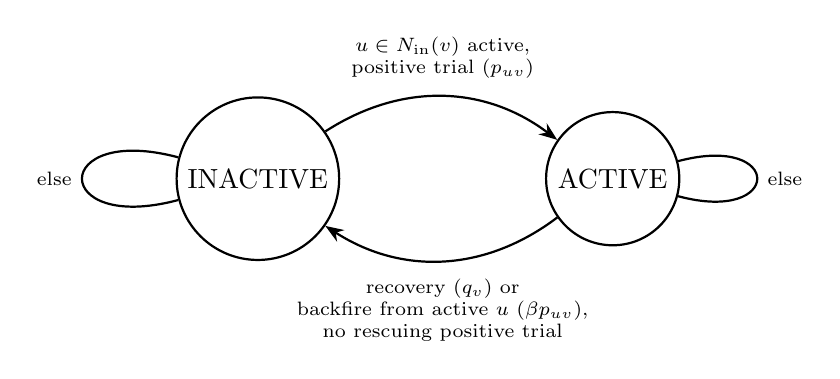
\begin{tikzpicture}[
  >=Stealth, node distance=2.6cm, thick,
  state/.style={circle, draw, minimum size=1.5cm, align=center},
  every loop/.style={min distance=10mm, looseness=8},
]
\node[state] (I) {INACTIVE};
\node[state, right=of I] (A) {ACTIVE};
\draw[->] (I) to[bend left=35] node[above=1mm, align=center, font=\scriptsize]
  {$u\in N_{\mathrm{in}}(v)$ active,\\positive trial ($p_{uv}$)} (A);
\draw[->] (A) to[bend left=35] node[below=1mm, align=center, font=\scriptsize]
  {recovery ($q_v$) or\\backfire from active $u$ ($\beta p_{uv}$),\\
  no rescuing positive trial} (I);
\path (I) edge[loop left, font=\scriptsize] node {else} (I);
\path (A) edge[loop right, font=\scriptsize] node {else} (A);
\end{tikzpicture}
}
\caption{Per-node round transition, illustrated for a single active
in-neighbor $u$ (the full rule, Eq.~(1), depends jointly on \emph{every}
active in-neighbor: any one successful positive trial rescues or
activates $v$, overriding recovery/backfire that same round).}
\label{fig:state-transition}
\end{figure}

The objective is cumulative expected spread,
\begin{equation}
f_\beta(S) \;=\; \mathbb{E}\Big[\sum_{t=1}^T |A_t|\Big], \qquad A_0=S,
\end{equation}
time-averaged spread being the same quantity up to the constant $1/T$.

\textbf{Fairness.} Let $u_g$ denote group $g$'s time-averaged realized reach
fraction (active fraction of $G_g$, averaged over rounds). Following an
isoelastic (constant elasticity of substitution) welfare
form~\cite{rahmattalabi2021fair}, define
\begin{equation}
W_\alpha(u) = \sum_g N_g\,\frac{u_g^\alpha}{\alpha}\ (\alpha\ne0), \qquad
W_0(u) = \sum_g N_g \log u_g,
\end{equation}
population-weighted by group size $N_g$; $\alpha\to1$ is utilitarian,
$\alpha=0$ is proportional fairness, and $\alpha\to-\infty$ approaches
leximin. As detailed in Section~\ref{sec:fairness-fix}, this project
identifies and corrects a measured pathology in the population-weighted
form and adopts, by default, the egalitarian (population-unweighted)
variant $W_\alpha(u)=\sum_g u_g^\alpha/\alpha$ instead, which counts each
group once regardless of size.

\section{Theoretical Results}
\label{sec:theory}

Statements below preserve the status labels of the underlying project
notes exactly: \emph{proven} (theorem, proposition, lemma, with a proof or
complete proof sketch), \emph{cited} (an external result relied upon), or
\emph{conjectural/conditional} (stated precisely, with the reason it is
not yet proven). No conjectural or conditional statement is used as a
premise for any theorem.

\subsection{Submodularity of the recovery-only process}

\begin{lemma}[Layered live-edge representation]
\label{lem:layered}
Fix $\beta=0$. Build a layered graph $\mathcal{L}$ on $V\times\{0,\dots,T\}$
with, for each round $t$, a self-edge $(v,t)\to(v,t{+}1)$ live iff
$R^t_v=0$, and a cross-edge $(u,t)\to(v,t{+}1)$ for each $(u,v)\in E$, live
iff $X^t_{uv}=1$. Then for every realization of the randomness,
$A_t = \{v : (v,t) \text{ reachable from } S\times\{0\}\text{ along live edges}\}$.
\end{lemma}
\emph{Proof.} By induction on $t$; at $t=0$ both sides equal $S$, and the
inductive step is exactly the layered-semantics transition rule read as a
reachability statement. $\blacksquare$

\begin{lemma}[Recovery alone preserves monotone submodularity]
\label{lem:recovery-submodular}
For $\beta=0$ and any recovery rates $q_v\in[0,1]$, $f_0(S)$ is monotone and
submodular in $S$.
\end{lemma}
\emph{Proof.} For each fixed realization, $|A_t|$ is the number of
layer-$t$ nodes reachable from $S\times\{0\}$ in a fixed DAG (Lemma~\ref{lem:layered}) --
a coverage function of $S$, hence monotone submodular; sums over $t$ and
expectations over realizations of monotone submodular functions remain
monotone submodular. $\blacksquare$

This isolates exactly which relaxation is "free": spontaneous,
state-independent recovery is harmless (it is a random self-edge and
reachability stays a coverage function), while neighbor-dependent
deactivation (backfire) destroys the coverage structure, since an active
in-neighbor can now \emph{remove} a node from the reachable set. This
sharpens the picture in Chan and Ning~\cite{chan2015influence}, who lose
submodularity under non-progressive \emph{threshold} rules where
deactivation depends on neighbor states; recovery alone needs no such
structure to stay submodular, on any graph.

\subsection{A sandwich approximation for all backfire intensities}

Let $U(S)\eqdef f_0(S)$ (the $\beta=0$ process at the true recovery rates).
For node $v$, let
$\delta_v \eqdef 1-\prod_{u\in N_{\mathrm{in}}(v)}(1-\beta p_{uv}) \le \beta\Delta_{\mathrm{in}}$,
where $\Delta_{\mathrm{in}}\eqdef\max_v\sum_{u\in N_{\mathrm{in}}(v)}p_{uv}$,
and let $L(S)$ be the $\beta=0$ process under inflated recovery
$q'_v\eqdef1-(1-q_v)(1-\delta_v)$.

\begin{lemma}[Upper coupling]
\label{lem:upper}
Under shared randomness, $A^\beta_t\subseteq A^0_t$ for all $t$; hence
$f_\beta(S)\le U(S)$.
\end{lemma}

\begin{lemma}[Lower coupling]
\label{lem:lower}
There is a coupling under which $A^L_t\subseteq A^\beta_t$ for all $t$;
hence $L(S)\le f_\beta(S)$.
\end{lemma}

Both couplings are proven by induction, replacing the per-edge backfire
trials with a single uniform draw compared against the aggregate kill
probability and, respectively, against $\delta_v$; the key inequality is
that $\beta$-kill implies $L$-extra-recovery because the $\beta$-kill
threshold is at most $\delta_v$ (attained when every in-neighbor is
active).

\begin{theorem}[Sandwich approximation, all $\beta$]
\label{thm:sandwich}
$L$ and $U$ are monotone submodular (Lemma~\ref{lem:recovery-submodular})
and $L\le f_\beta\le U$ pointwise (Lemmas~\ref{lem:upper}--\ref{lem:lower}).
Let $S_L, S_U$ be the greedy solutions for $L, U$ under $|S|\le k$, $S_\beta$
the greedy solution run directly on $f_\beta$, and
$S_{\mathrm{sand}}=\arg\max_{S\in\{S_L,S_U,S_\beta\}} f_\beta(S)$. Then, with
$S^\star$ optimal for $f_\beta$,
\begin{equation}
\begin{split}
f_\beta(S_{\mathrm{sand}}) &\ge \max\left\{\frac{f_\beta(S_U)}{U(S_U)},\ \frac{L(S^\star)}{f_\beta(S^\star)}\right\}\Big(1-\frac1e\Big) f_\beta(S^\star)\\
&\ge \rho\Big(1-\frac1e\Big)\mathrm{OPT}_\beta,
\end{split}
\end{equation}
where $\rho \eqdef \min_{|S|\le k} L(S)/U(S)$.
\end{theorem}
\emph{Proof.} Cited: the sandwich-approximation theorem of Lu, Chen, and
Lakshmanan~\cite{lu2015competition}, applied to the bracket $L\le f_\beta\le U$;
the $(1-1/e)$ factors are~\cite{nemhauser1978analysis} applied to greedy on
each submodular surrogate. The final inequality follows from
$L(S^\star)/f_\beta(S^\star)\ge L(S^\star)/U(S^\star)\ge\rho$. $\blacksquare$

Theorem~\ref{thm:sandwich} improves on treating backfire as an arbitrary
perturbation from submodularity via~\cite{horel2016maximization}, which
would only hold for $\beta=O(n^{-1/2})$ -- far below the
$\beta\in[0.1,0.7]$ regime our empirical study targets -- because it
exploits the \emph{structure} of the perturbation (a bounded extra kill
rate) rather than treating it adversarially, and it holds for every
$\beta$, recovering the tight $(1-1/e)$ exactly at $\beta=0$ (where $L=U$,
$\rho=1$). It also yields a practical corollary: since $L$ and $U$ are
ordinary $\beta=0$ processes that can be simulated directly, $f_\beta(S)/U(S)$
is a directly computable, per-instance certificate,
$f_\beta(S)\ge \frac{f_\beta(S)}{U(S)}(1-\frac1e)\mathrm{OPT}_\beta$ -- the
algorithm ships its own approximation guarantee on every instance it is run
on.

\begin{proposition}[Finite-horizon bound on $\rho$]
\label{prop:rho-bound}
$\rho \ge (1-\beta\Delta_{\mathrm{in}})^T$.
\end{proposition}
This is proven by charging every self-edge of a witness reachability path
under the coupling of Lemma~\ref{lem:lower}, and is conservative (it ignores
re-activation through alternate paths). A tighter steady-state conjecture,
$\rho \gtrsim q/(q+\beta\Delta_{\mathrm{in}})$ for $q=\min_v q_v$, is stated
in the underlying project notes as an explicit \emph{conjecture}: the
heuristic single-sojourn argument does not account for the downstream
cascade a shortened sojourn fails to seed, and closing that gap is left
open. This conjecture is not used in any proof in this paper (Section~\ref{sec:limitations}
discusses why it is, in any case, not the most promising target for
tightening the sandwich ratio).

\subsection{A closed-form index for the control problem}
\label{sec:index}

Given the mean-field belief field (Section~\ref{sec:algorithm}), each
node's per-round control problem is a 2-state MDP -- states
$s\in\{0,1\}$, discount $\gamma$, reward $w$ at $s=1$ -- with natural
transitions $a=p_{01}$ (activate), $b=p_{10}$ (deactivate), and three
actions: NONE (free, either state), CONVERT (cost $c_C$, forces $0\to1$,
only at $s=0$), MAINTAIN (cost $c_M$, forces stay-at-1, only at $s=1$),
under a shared Lagrange price $\lambda$ per unit cost. There are exactly
four deterministic stationary policies, named by (action at 0, action at
1): NN, NM, CN, CM. Figure~\ref{fig:mdp} shows this per-node MDP; the
index $\lambda^\star_v$ of Proposition~\ref{prop:indexability} below is
computed from it in closed form, once per node, every round.

\begin{figure}[t]
\centering
\resizebox{0.85\columnwidth}{!}{
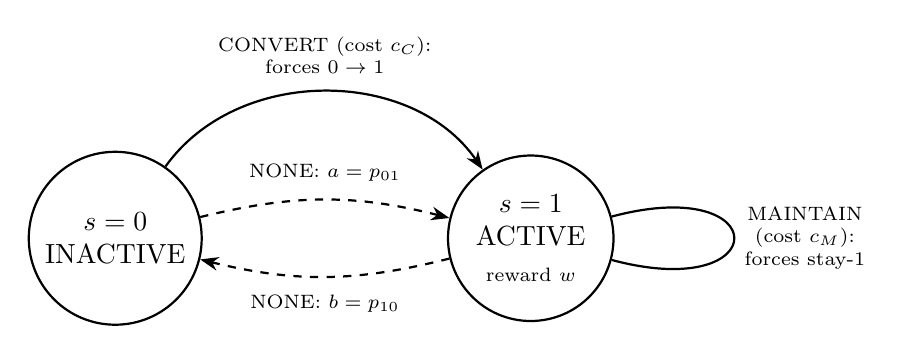
\begin{tikzpicture}[
  >=Stealth, node distance=3.1cm, thick,
  state/.style={circle, draw, minimum size=1.3cm, align=center},
]
\node[state] (S0) {$s=0$\\INACTIVE};
\node[state, right=of S0] (S1) {$s=1$\\ACTIVE\\[1pt]{\scriptsize reward $w$}};
\draw[->] (S0) to[bend left=55] node[above=1mm, align=center, font=\scriptsize]
  {CONVERT (cost $c_C$):\\forces $0\to1$} (S1);
\draw[->, dashed] (S0) to[bend left=14] node[above=1mm, align=center, font=\scriptsize]
  {NONE: $a=p_{01}$} (S1);
\draw[->, dashed] (S1) to[bend left=14] node[below=1mm, align=center, font=\scriptsize]
  {NONE: $b=p_{10}$} (S0);
\path (S1) edge[loop right, min distance=14mm, looseness=10, font=\scriptsize]
  node[align=center] {MAINTAIN\\(cost $c_M$):\\forces stay-1} (S1);
\end{tikzpicture}
}
\caption{The per-node 2-state/3-action MDP each round's index computation
solves (dashed: unpaid natural transitions; solid: the two paid, forced
actions). Section~\ref{sec:index} gives the four resulting stationary
policies' closed-form value functions and the resulting index
$\lambda^\star_v$.}
\label{fig:mdp}
\end{figure}

\begin{proposition}[Closed forms]
\label{prop:closedform}
With $D\eqdef(1-\gamma)(1-\gamma+\gamma(a+b))$, each policy's value
functions $V_1(\lambda), V_0(\lambda)$ are given in closed, affine-in-$\lambda$
form by solving its fixed $2\times2$ linear system (e.g., for CN,
$V_0=-\lambda c_C+\gamma V_1$ and $V_1=w+\gamma[(1-b)V_1+bV_0]$, giving
$V_1=(w-\gamma b\lambda c_C)/((1-\gamma)(1+\gamma b))$); the full table of
four closed forms is given in the underlying project notes and reproduced
in the algorithm's implementation.
\end{proposition}

\begin{proposition}[Convexity in $\lambda$]
\label{prop:convexity}
$V^*(s,\lambda)=\max_\pi V_\pi(s,\lambda)$ over the four policies is a
maximum of four affine functions of $\lambda$: convex, piecewise linear,
with at most three breakpoints, computable in $O(1)$.
\end{proposition}
\emph{Proof.} In a discounted finite MDP some stationary deterministic
policy is optimal at every state simultaneously, so $V^*$ is exactly this
finite max; Killian, Perrault, and Tambe~\cite{killian2021beyond} (their
Prop.\ 4.1) prove convexity in $\lambda$ for the general multi-action
restless-bandit case, of which this is a one-line special case via finite
enumeration of the four policies. $\blacksquare$

\begin{proposition}[Index and indexability, this case]
\label{prop:indexability}
Define node $v$'s index $\lambda^\star_v$ as the largest $\lambda\ge0$ at
which the optimal policy still takes the paid action at $v$'s current state.
\end{proposition}
A proof \emph{sketch} shows the paid action's advantage over NONE has a
strictly negative slope in $\lambda$ from the cost term, while the value
gap $V^*_1-V^*_0$ is non-increasing in $\lambda$ on each linear piece,
checked by finite case analysis over the four policies. \textbf{We state
plainly, matching the underlying project notes' own status label, that
indexability -- i.e., that the paid set is a down-set $[0,\lambda^\star_v]$
-- is only verified numerically here} (on random instances, over a fine
$\lambda$ grid, checking that per-node cost is non-increasing in
$\lambda$), not proven in general; the finite four-policy structure makes
this tractable to check exactly where Killian et
al.~\cite{killian2021beyond} call general multi-action indexability
"notoriously difficult" and avoid it. The index itself is defined as the
supremum of the paid set, which remains well-defined and exactly computable
regardless.

\begin{theorem}[Per-round complexity]
\label{thm:complexity}
Given Propositions~\ref{prop:closedform}--\ref{prop:indexability}, one
round of the control policy costs $O(Km+n\log n)$, where $K$ is the number
of mean-field fixed-point iterations (geometric convergence under a
contraction condition on $\Delta\max(p^+,p^-)$).
\end{theorem}
The $n\log n$ term sorts nodes by $\lambda^\star_v$ and fills the shared
budget greedily -- exactly "smallest $\lambda$ with aggregate cost
$\le B$," the target of the bisection-plus-value-iteration procedure it
replaces, which cost $O(n\cdot I_{\mathrm{bisect}}\cdot I_{\mathrm{VI}})$
(on the order of $8000\,n$ scalar operations per round in our
configuration); this project's own measurements put the closed-form
replacement at roughly $130\times$ faster per round than that bisection
oracle. For comparison, naive Monte Carlo KKT greedy costs $O(knRm)$ per
seed set, and one static IMM selection costs
$O((k+\ell)(n+m)\log n/\varepsilon^2)$~\cite{tang2015influence}: our
per-round cost is near-linear like a single IMM run but is paid $T$ times,
the stated price of sustaining influence under decay rather than seeding
once.

\subsection{Hardness}
\label{sec:hardness}

For $\beta=0$ (and $q=0$, large $T$), the problem contains max-$k$-cover, so
$1-1/e$ is an unbeatable ceiling for every $\beta\ge0$ under
$\mathrm{P}\ne\mathrm{NP}$~\cite{feige1998threshold,nemhauser1978analysis} --
adding backfire cannot remove hard instances on which $\beta$ is simply
irrelevant. For adversarial, arbitrary non-submodular perturbations, no
constant-factor approximation exists in general once a function is
$\omega(n^{-1/2})$-far from submodular~\cite{horel2016maximization};
Theorem~\ref{thm:sandwich} escapes this only because our perturbation is
structured, not adversarial.

\begin{theorem}
\label{thm:hardness}
For every fixed $\beta\in[0,1)$, no polynomial-time algorithm approximates
$f_\beta$ within $(1-1/e+\varepsilon)$ for any $\varepsilon>0$ unless
$\mathrm{P}=\mathrm{NP}$.
\end{theorem}
\emph{Proof.} Reduction from max-$k$-cover,
$(1-1/e+\varepsilon)$-inapproximable unless
$\mathrm{P}=\mathrm{NP}$~\cite{feige1998threshold}. Build a bipartite
digraph (set-nodes to element-nodes, edge probability 1), each element
replicated to swamp the additive seed-count term. The key subtlety is that
backfire \emph{is} realized on this instance (a seed keeps attacking every
element it covers), so its harmlessness must be shown, not assumed. On this
instance class, an element with $c\ge1$ active covering seeds throughout is
a two-state chain with up-rate 1 and down-rate $1-(1-\beta)^c$, giving an
exact value formula
$f_\beta(S)=kT+T\sum_v\varphi_\beta(c_v(S))+O(n)$ with
$\varphi_\beta(c)=1/(2-(1-\beta)^c)$ strictly decreasing in $c\ge1$ and
bounded below by $1/2$; the max-coverage gap therefore survives backfire
intact. $\blacksquare$

This value formula also shows $f_\beta\ge f_0/2$ for \emph{every} seed set
on this instance class at $q=0$, exactly where the sandwich ratio $\rho$ of
Theorem~\ref{thm:sandwich} is vacuous ($\rho=0$).

A natural next question is whether backfire forces a further,
$\beta$-dependent worsening \emph{beyond} $1-1/e$. We do not claim such a
result here: a candidate constant $c(\beta)\in[0.94,1)$ is derivable under
one extra, unverified property of Feige's hard instances, but proving that
property would require re-deriving part of Feige's reduction, which we
have not done to a standard we are willing to publish as a theorem. We
report this only as an open conjecture, with supporting (not conclusive)
structural and numerical evidence, in
Section~\ref{sec:limitations}.

\section{Algorithm: MF-BWI-Fair}
\label{sec:algorithm}

MF-BWI-Fair (Mean-Field Belief with a Lagrangian index and isoelastic-Welfare
reweighting, Fair) is a stateful per-round control policy summarized in
Figure~\ref{fig:pipeline}. Each round:

\begin{enumerate}
\item \textbf{Bayesian posterior tracking.} A Beta--Bernoulli tracker
  maintains posterior means $\hat p_{uv}^+, \hat p_{uv}^-, \hat q_v$ for
  every edge/node from observed trial outcomes; the policy never sees the
  simulator's hidden true parameters, only these running estimates.
\item \textbf{Mean-field belief fixed point.} Exact per-node marginals
  require tracking correlations across the whole active-set distribution,
  intractable at scale. We use the standard individual-based / N-intertwined
  mean-field approximation from network epidemic models: each node's
  in-neighbors are replaced by their marginal activation probabilities
  $m_u$, giving the self-consistency equation
  \begin{equation}
  \begin{split}
  m_v = m_v(1-\hat q_v)\!\!\prod_{u\in N_{\mathrm{in}}(v)}\!\!(1-\hat p^-_{uv}m_u) \\
  {}+(1-m_v)\Big(1-\!\!\prod_{u\in N_{\mathrm{in}}(v)}\!\!(1-\hat p^+_{uv}m_u)\Big),
  \end{split}
  \end{equation}
  solved by Jacobi fixed-point iteration to tolerance $10^{-4}$ or 50
  iterations. We verified directly that the alternative network-coupling
  method of Ou et al.~\cite{ou2022networked} does not apply here, since it
  requires a deterministic action-vector coupling rather than the
  genuinely bilinear neighbor-\emph{state} coupling this model has.
\item \textbf{Group welfare weights.} Each group's current marginal
  welfare weight $w_g$ is computed from its tracked time-averaged realized
  reach $u_g$ (Section~\ref{sec:fairness-fix}), egalitarian by default.
\item \textbf{Closed-form Lagrangian index.} Using the converged belief
  field to obtain each node's "no-action" transition probabilities
  $p_{01}(v), p_{10}(v)$, each node's 2-state/3-action MDP is built with
  reward $r_v(s)=w_{g(v)}\cdot s$, and the shared-budget Lagrangian
  relaxation is solved via the closed-form index of
  Section~\ref{sec:index} (a bisection-plus-value-iteration oracle is kept
  as a test reference).
\item \textbf{Leftover-budget fill.} Any budget left over from the index
  scan's discreteness is filled by a greedy tie-break on each node's
  closed-form index (or Bellman gap, under the bisection oracle), keeping
  the hard budget constraint intact without reintroducing per-group floors
  or quotas.
\item \textbf{Execute, observe, update.} Actions are applied; the simulator
  advances one round under the layered-semantics transition rule
  (Section~\ref{sec:model}); observed trial outcomes update the Bayesian
  tracker; and each group's realized reach average $u_g$ is updated for the
  next round's weights.
\end{enumerate}

\begin{figure}[t]
\centering
\resizebox{\columnwidth}{!}{
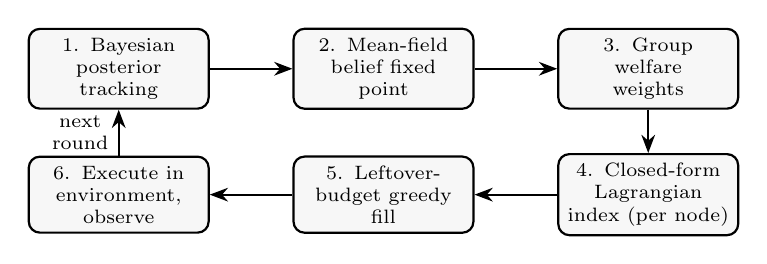
\begin{tikzpicture}[
  >=Stealth, node distance=0.55cm and 1.05cm, thick, font=\scriptsize,
  box/.style={draw, rounded corners, align=center, minimum height=0.9cm, text width=2.05cm, fill=black!3},
]
\node[box] (bayes) {1. Bayesian\\posterior\\tracking};
\node[box, right=of bayes] (mf) {2. Mean-field\\belief fixed\\point};
\node[box, right=of mf] (fair) {3. Group\\welfare\\weights};
\node[box, below=of fair] (index) {4. Closed-form\\Lagrangian\\index (per node)};
\node[box, left=of index] (fill) {5. Leftover-\\budget greedy\\fill};
\node[box, left=of fill] (env) {6. Execute in\\environment,\\observe};
\draw[->] (bayes) -- (mf);
\draw[->] (mf) -- (fair);
\draw[->] (fair) -- (index);
\draw[->] (index) -- (fill);
\draw[->] (fill) -- (env);
\draw[->] (env.north) -- (bayes.south) node[midway, left, align=center] {next\\round};
\end{tikzpicture}
}
\caption{MF-BWI-Fair's per-round control loop (numbered as in the list
above); Algorithm~\ref{alg:mfbwi} gives the corresponding pseudocode.}
\label{fig:pipeline}
\end{figure}

\begin{algorithm}[t]
\caption{MF-BWI-Fair, one round}
\label{alg:mfbwi}
\begin{algorithmic}[1]
\REQUIRE graph $G$, state $s$, budget $B$, fairness exponent $\alpha$
\STATE $(\hat p^+,\hat p^-,\hat q) \gets$ posterior means from tracker
\STATE $m \gets$ mean-field fixed point of Eq.~(5) from $(s,\hat p^+,\hat p^-,\hat q)$
\STATE $(p_{01}, p_{10}) \gets$ field transition probabilities from $m$
\STATE $u \gets$ tracked per-group time-averaged reach
\STATE $w \gets$ \textsc{GroupWelfareWeights}$(u, \alpha)$ \hfill (egalitarian default)
\FOR{each node $v$}
  \STATE build 2-state/3-action MDP with reward $w_{g(v)}\cdot s_v$, kernel $(p_{01}(v), p_{10}(v))$
  \STATE $\lambda^\star_v \gets$ closed-form index (Prop.~\ref{prop:indexability})
\ENDFOR
\STATE sort nodes by $\lambda^\star_v$ descending; select prefix fitting in $B$
\STATE greedily fill leftover budget by descending index among unselected nodes
\STATE apply CONVERT/MAINTAIN to selected nodes, NONE elsewhere
\STATE observe transition, update Bayesian tracker and $u_g$
\end{algorithmic}
\end{algorithm}

\subsection{The fairness fix: population-weighted vs.\ egalitarian welfare}
\label{sec:fairness-fix}

Rahmattalabi et al.'s isoelastic welfare weight, implemented exactly as
published, is $w_g=N_g u_g^{\alpha-1}$ (or $N_g/u_g$ at $\alpha=0$): the
correct marginal utility for maximizing \emph{aggregate} welfare, in which
a group's contribution scales with its population. This has a concrete,
measured downside for the stated goal of not neglecting a small group: at
$\alpha=0$, group $g$'s weight exceeds group $g'$'s only once
$u_{g'}/u_g > N_{g'}/N_g$ -- the smaller group must be under-served by a
factor proportional to the group-size \emph{ratio} before the mechanism
reacts at all. On this project's own three-group (20/40/60) benchmark
graph, at a neutral $\alpha_{\mathrm{fair}}=0$ this kept the smallest group
at a visibly lower realized reach than the largest purely because a
$3\times$ reach gap was required before the weight formula began favoring
it. We therefore adopt, as the default, the egalitarian
(population-unweighted) form $w_g=u_g^{\alpha-1}$ (or $1/u_g$ at
$\alpha=0$), a standard alternative welfare form in the social-welfare and
fair-division literature (not a new mechanism), counting each group once
regardless of size -- the appropriate choice when fairness means each
\emph{group}, not each person, is treated fairly regardless of population.

\section{Experimental Setup}
\label{sec:setup}

\textbf{Graph.} The primary validation graph is a single synthetic
stochastic block model with three groups of unequal size (20/40/60, 120
nodes total), within-block edge probability $p_{\mathrm{in}}=0.07$,
between-block edge probability $p_{\mathrm{out}}=0.008$, and per-edge
positive-influence probability $p_{uv}\sim\mathrm{Uniform}(0.05,0.15)$.
Density was hand-tuned so the network neither saturates near full
activation nor fails to cascade at all, either of which would mask the
effects under study. This is the primary benchmark reported in
Section~\ref{sec:results-main}; Section~\ref{sec:results-multigraph}
additionally reports the same six-algorithm comparison on three further
synthetic graphs at different scales and topologies and on three real
social networks, checking that the main benchmark's qualitative finding
does not depend on this one hand-tuned graph. A fourth, larger synthetic
graph targeting a more specific follow-up question is introduced later,
in Section~\ref{sec:limitations}.

\textbf{Budget and horizon.} Per-round budget $B=100$, horizon $T=30$
rounds. One-shot baselines are given $k=20$ seeds, chosen so that
$k\cdot\mathrm{cost}(\mathrm{CONVERT})=100=B$: one round's worth of
MF-BWI-Fair's budget, spent once at round 0.

\textbf{Baselines.} \emph{KKT-greedy/CELF}~\cite{kempe2003maximizing,leskovec2007cost}:
classical Monte Carlo greedy under plain progressive IC ($\beta=0$, $q=0$),
this project's own reimplementation, used as the "ignore all four
relaxations" ablation. \emph{Fair-greedy}: an in-house welfare-weighted
greedy baseline in the style of~\cite{rahmattalabi2021fair} maximizing a
sum of concave per-group log-utilities. \emph{Repeated-greedy}: an in-house
cost-effective greedy that re-selects actions every round under the same
per-round budget, using \emph{true} parameters directly (no Bayesian
uncertainty, no fairness mechanism) -- the strongest plausible classical
competitor that also acts repeatedly, included specifically to isolate
whether MF-BWI-Fair's advantage is more than "gets to act every round."
\emph{IMM}~\cite{tang2015influence}: this project's independent
reimplementation of the two-phase martingale sampling and node-selection
algorithm, cross-checked against the paper's own pseudocode and against a
documented erratum~\cite{chen2018issue}. \emph{He--Kempe Saturate
Greedy}~\cite{he2016robust}: this project's independent reimplementation of
the bicriteria robust algorithm, given the low/high corners of the
$p_{uv}$ range as its scenario set. \emph{MF-BWI-Fair}, as described in
Section~\ref{sec:algorithm}.

\textbf{Honesty notes on baseline provenance.} Other than the objective
forms they target, every baseline in this comparison is an
independently-verified reimplementation, not the original authors' code.
Official code exists for IMM (a SourceForge project by the original
authors) and no official code was found for He--Kempe's Saturate Greedy or
for Rahmattalabi et al.'s welfare mechanism specifically. All IMM numbers
reported here are from this project's own Python reimplementation; we
additionally benchmark that reimplementation directly against the original
authors' C++ implementation and report the outcome in
Section~\ref{sec:results-imm}. No equivalent direct comparison
exists for He--Kempe or Rahmattalabi et al.'s mechanisms, since no official
code was found for either; those numbers remain characterizations of this
project's own reimplementations only, cross-checked against the papers'
stated algorithms and theorem statements, not the original authors'
published numbers.

\textbf{Metrics.} (a) time-averaged active-node count over the full
horizon; (b) per-group reach fraction (own-group-size-normalized,
time-averaged) and its minimum across groups; (c) wall-clock runtime.
Sweeps are conducted over backfire intensity $\beta$, recovery rate $q$,
and the fairness exponent $\alpha_{\mathrm{fair}}$, each with 15
independent trials using common random numbers across the swept parameter
within a trial to reduce sweep-trend noise without narrowing between-trial
variance.

\section{Results}
\label{sec:results}

\subsection{Main benchmark: a 120-node stochastic block model}
\label{sec:results-main}

Table~\ref{tab:main-spread} reports time-averaged spread for all six
algorithms at the extremes of the backfire ($\beta$) and recovery ($q$)
sweeps described in Section~\ref{sec:setup}, as mean $\pm$ half-width of
a 95\% confidence interval over the 15 trials. Figure~\ref{fig:main-sweeps}
shows the full sweep rather than just these three points, and confirms
the same pattern holds in between. At $\beta=0$, $q=0.05$, close to the
plain progressive-IC setting every one-shot baseline targets,
Lemma~\ref{lem:recovery-submodular} guarantees that neither MF-BWI-Fair
nor repeated-greedy can exceed the proven $(1-1/e)$ ceiling, regardless of
$q$; consistent with that, a paired Wilcoxon signed-rank test finds them
statistically indistinguishable there ($W=49$, $p=0.53$, $n=15$). Once
either $\beta$ or $q$ departs from its low end, MF-BWI-Fair opens a lead
over every other algorithm that is both large and statistically
significant: the same paired test rejects equality against
repeated-greedy and against the best one-shot baseline at every other
column and sweep point we checked ($p<0.001$ in every case), and the
lead reaches more than $6\times$ the best one-shot baseline's spread at
$q=0.4$.

\begin{table}[t]
\centering
\caption{Time-averaged spread, 120-node SBM benchmark: mean $\pm$
half-width of a 95\% CI over 15 trials. SG = He--Kempe's Saturate Greedy.}
\label{tab:main-spread}
\footnotesize
\setlength{\tabcolsep}{2.5pt}
\begin{tabular}{lccc}
\toprule
Algorithm & $\beta{=}0,q{=}0.05$ & $\beta{=}0.7,q{=}0.05$ & $\beta{=}0.15,q{=}0.4$ \\
\midrule
KKT-greedy/CELF   & 78.0$\pm$1.9  & 50.8$\pm$1.9  & 11.8$\pm$2.1 \\
Fair-greedy       & 78.4$\pm$2.2  & 52.6$\pm$2.2  & 13.7$\pm$2.3 \\
IMM               & 77.7$\pm$2.1  & 53.1$\pm$2.2  & 15.7$\pm$2.6 \\
He--Kempe SG      & 72.8$\pm$1.9  & 48.9$\pm$2.4  & 12.2$\pm$2.6 \\
Repeated-greedy   & \textbf{108.8}$\pm$0.5 & 96.3$\pm$1.2  & 77.2$\pm$1.9 \\
MF-BWI-Fair       & \textbf{108.5}$\pm$0.5 & \textbf{104.6}$\pm$0.5 & \textbf{102.0}$\pm$0.5 \\
\bottomrule
\end{tabular}
\end{table}

We bold both column-1 entries deliberately, since the 0.3-point gap
between them is well inside the pair's own trial-to-trial noise: their
95\% CIs overlap almost entirely, and the paired test above finds no
significant difference. This matches the $(1-1/e)$-tie the theory
predicts at this point, so we report it as a tie, not as an unresolved
discrepancy.

\begin{figure}[t]
\centering
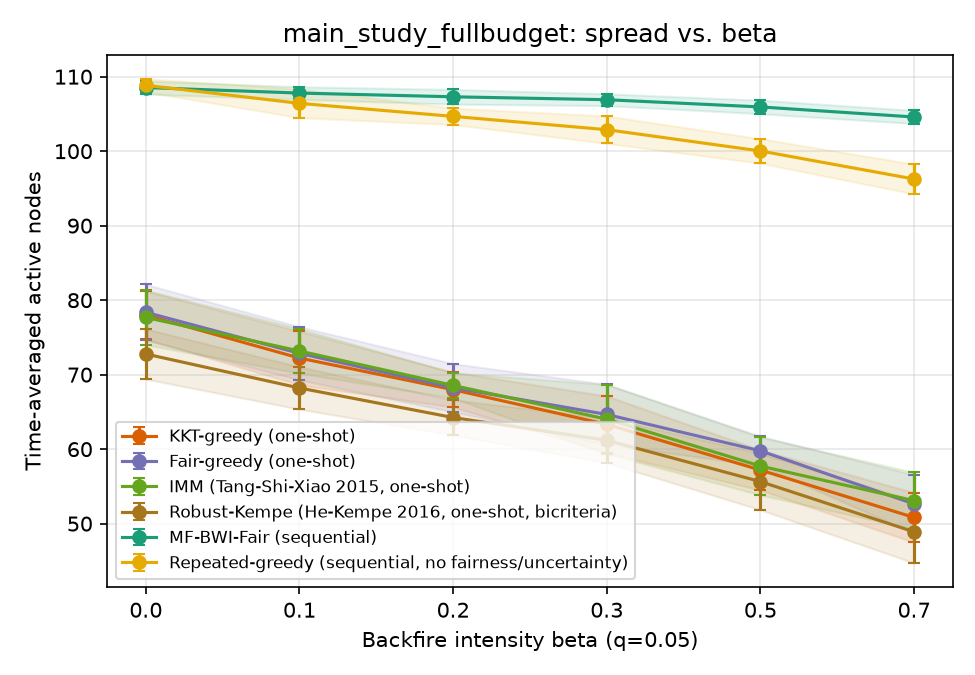
\includegraphics[width=\columnwidth]{figures/main_beta_sweep.png}
\\[4pt]
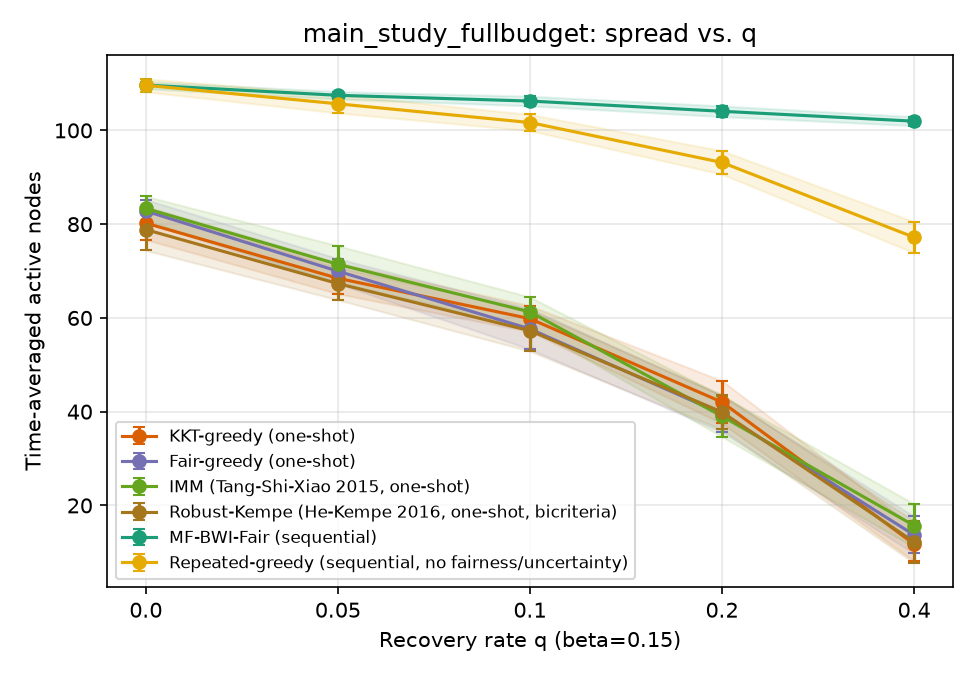
\includegraphics[width=\columnwidth]{figures/main_q_sweep.png}
\caption{Full sweeps underlying Table~\ref{tab:main-spread} (mean $\pm$
95\% CI shading, 15 trials per point): time-averaged spread vs.\ backfire
intensity $\beta$ at $q=0.05$ (top) and vs.\ recovery rate $q$ at
$\beta=0.15$ (bottom), all six algorithms. Both sweeps show the same
shape reported in the text at the three extreme points: MF-BWI-Fair
statistically tied with repeated-greedy at the low end and opening a
significant, growing lead as either parameter increases, with the four
one-shot baselines clustered well below both throughout.}
\label{fig:main-sweeps}
\end{figure}

The four one-shot classical baselines (KKT-greedy, Fair-greedy, IMM,
He--Kempe robust) cluster together throughout, as expected: none of them
is designed to act more than once or to track a changing state, so all
four degrade together as backfire/recovery intensify, regardless of
which classical guarantee they individually carry. He--Kempe's Saturate
Greedy is consistently the weakest of the four (it hedges against a
worst-case scenario corner that never actually realizes in this
benchmark, spending roughly 25\% fewer seeds -- about 15 of the
$K=20$ budget -- to do so); this is the correct, expected behavior of a
robustness guarantee under a benign instance, not a defect. MF-BWI-Fair's
margin over He--Kempe specifically is the cleanest evidence that
\emph{paying for robustness against a probability range} and
\emph{adaptively learning the realized value inside that range} are not
the same thing: MF-BWI-Fair beats He--Kempe by a wide margin even at
$\beta=0$, $q=0.05$ (108.5 vs.\ 72.8), where it is merely tied with
repeated-greedy.

Fairness (min-group reach, the minimum own-group-normalized reach across
groups) tells a related story once the population-weighting pathology in
the isoelastic welfare objective is corrected (Section~\ref{sec:algorithm}):
at the neutral default, MF-BWI-Fair matches or leads repeated-greedy's
min-group reach almost everywhere ($\beta=0$: 0.888 vs.\ 0.880; $\beta=0.7$:
0.809 vs.\ 0.781; $q=0.4$: 0.826 vs.\ 0.590), with a single small residual
gap at $q=0$ (0.895 vs.\ 0.898). Total spread is essentially unchanged by
the fairness correction, so this is a genuine improvement in the
default operating point rather than a trade-off paid for it. The
$\alpha_{\mathrm{fair}}$ knob provides an additional, independent lever
on top of this default. Min-group reach trends upward from 0.809 at the
utilitarian extreme ($\alpha_{\mathrm{fair}}=1$) to 0.859 at a
leximin-like extreme ($\alpha_{\mathrm{fair}}=-8$), and it crosses
repeated-greedy's fixed 0.817 near $\alpha_{\mathrm{fair}}\approx0.5$.
This trend is not perfectly monotonic at every intermediate point:
$\alpha_{\mathrm{fair}}=0.5$ shows a local peak of 0.863, and
$\alpha_{\mathrm{fair}}=0$ a local dip to 0.829. We attribute these
intermediate wiggles to trial noise, since they fall inside the
15-trial confidence intervals rather than reversing the overall trend.
Total spread likewise trends higher, from 105.8 to 107.6, rather than
falling across the same range, so fairness and spread are not in tension
in this benchmark, even though neither quantity moves perfectly
monotonically at every intermediate $\alpha_{\mathrm{fair}}$ value
tested. On the runtime axis, the
closed-form Lagrangian index (Section~\ref{sec:algorithm}) is
approximately $130\times$ faster per per-round decision than the
bisection-plus-value-iteration procedure it replaces, at identical
output (verified on matched inputs), making MF-BWI-Fair's per-round cost
$O(Km+n\log n)$ rather than the multiplicatively more expensive
bisection oracle.

\subsubsection{Runtime scaling}
\label{sec:results-scaling}
Every experiment above uses graphs of at most 532 nodes, the largest
real graph in Section~\ref{sec:results-multigraph}. That scale is too
small to stress-test the $O(Km+n\log n)$ per-round complexity claimed in
Theorem~\ref{thm:complexity}, so we separately measure MF-BWI-Fair's
wall-clock per-round decision time on Barabasi--Albert graphs from
$n=100$ to $n=100{,}000$ nodes, holding average degree fixed at
$\approx6$ ($m=3$ attachments) so that the measurement isolates the
$n$-dependence from degree effects. Figure~\ref{fig:scaling} shows the
result. Per-round time grows from 0.013s at $n=100$ to 43.8s at
$n=100{,}000$; a least-squares fit in log-log space gives an empirical
power law of $O(n^{1.30})$ over $n\in[1000,100{,}000]$, mildly
superlinear rather than the pure linear-in-$n$ behavior a reader might
expect from a casual reading of $O(Km+n\log n)$ with $m=O(n)$ at fixed
average degree. This does not violate Theorem~\ref{thm:complexity},
because the theorem leaves $K$ (the number of mean-field fixed-point
iterations to converge) as a separate, instance-dependent factor and
never asserts $K=O(1)$. We think the most plausible explanation is
structural: Barabasi--Albert graphs' heavy-tailed degree distribution
produces a small number of increasingly high-degree hub nodes as $n$
grows, and these hubs mildly weaken the fixed point's contraction rate,
which in turn mildly increases $K$ with $n$ on this specific graph
family. We report this as a real, disclosed effect rather than as a
claimed $O(n)$ result, and we leave a fuller characterization of $K$'s
own graph-family dependence to future work. Even with this caveat, the
measured cost remains dramatically more favorable than the classical
alternatives compared against in Section~\ref{sec:index}: naive Monte
Carlo KKT-greedy's $O(knRm)$ per seed set is untenable at
$n=100{,}000$, since a single seed selection would already require on
the order of $k\cdot n\cdot R$ full-graph passes, whereas MF-BWI-Fair
completes a full per-round decision in under a minute at this scale on
ordinary hardware, with no GPU or distributed infrastructure.

\begin{figure}[t]
\centering
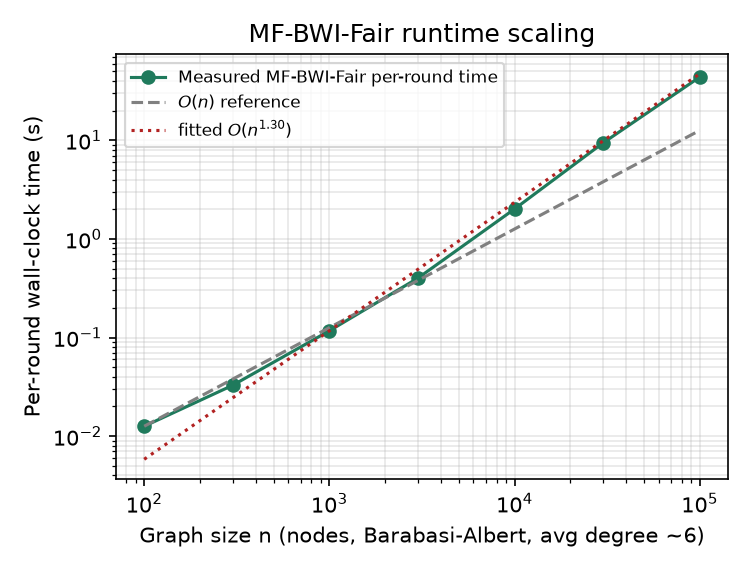
\includegraphics[width=\columnwidth]{figures/runtime_scaling.png}
\caption{MF-BWI-Fair per-round wall-clock time vs.\ graph size $n$
(Barabasi--Albert, average degree $\approx6$, log-log axes), against an
$O(n)$ reference line and the fitted $O(n^{1.30})$ power law.}
\label{fig:scaling}
\end{figure}

\subsection{Multi-graph and real-network validation}
\label{sec:results-multigraph}

The benchmark above uses a single hand-tuned synthetic graph. We validate
generalization on three further synthetic graphs -- \texttt{small\_sbm}
(60 nodes), \texttt{large\_sbm} (240 nodes, double every block size of the
main benchmark), and \texttt{barabasi\_albert} (150 nodes, a structurally
different scale-free topology) -- and on three real social networks at
increasing scale, all connected friendship subgraphs from the SNAP
ego-Facebook dataset~\cite{mcauley2012learning}: \texttt{real\_facebook\_348}
(224 nodes, 6{,}384 edges), \texttt{real\_facebook\_686} (168 nodes,
3{,}312 edges), and \texttt{real\_facebook\_3437} (532 nodes, 9{,}624
edges, the sparsest and most community-structured of the three, with 6
detected communities of sizes 39--165) (Weighted-Cascade edge
probabilities~\cite{chen2009efficient}, and community-detection-derived
groups as a structural fairness proxy in the absence of demographic
attributes).

\textbf{The synthetic-graph finding reproduces across scale and topology.}
On all three additional synthetic graphs, MF-BWI-Fair is tied with
repeated-greedy at $\beta=q=0$ and opens a clear, growing lead as $\beta$
or $q$ increases, in both spread and min-group reach -- e.g.\
\texttt{large\_sbm} at $q=0.4$: 202.8 vs.\ 164.2 spread ($+23\%$);
\texttt{small\_sbm} at $q=0.4$: min-group reach 0.772 vs.\ 0.553. This
result is not an artifact of the one hand-tuned 120-node graph used for
the main benchmark. A fourth synthetic graph, \texttt{large\_community\_sbm}
(1,065 nodes, six disparately-sized communities), targets a more specific
question and is discussed with the real-graph exception in
Section~\ref{sec:limitations}.

\textbf{The real network initially diverged; restoring compute budget and
fixing a harness bug both mattered, and together resolve it.} At a
necessarily reduced compute budget (shorter horizon, smaller $K$/$B$,
fewer Monte Carlo samples, and critically a cut-down 1-rollout
repeated-greedy instead of its 2-rollout library default -- required to
keep runtime tractable at \texttt{real\_facebook\_348}'s $\sim\!28.5$
average degree, 4--9$\times$ every synthetic graph tested), MF-BWI-Fair
did \emph{not} show the dominant advantage seen on every synthetic graph:
it trailed repeated-greedy by 2--11\% in spread at every checkpoint tested
and showed a mixed, sometimes clearly worse, min-group reach (e.g.\
$\beta=0.5$: 0.351 vs.\ 0.474, a 26\% deficit). We report this plainly,
as an honest negative finding, rather than omitting it. Re-running the
identical graph with compute budget fully restored to the main
benchmark's settings ($T=30$, $B=100$, $K=20$, 15 trials, full Monte
Carlo sample counts, repeated-greedy's own 2-rollout default)
flips every one of the four original checkpoints from ``MF-BWI-Fair
behind'' to ``tied or ahead'' (Table~\ref{tab:realgraph}), confirming
budget was the dominant cause of the initial divergence on this graph.

Extending the same full-budget protocol to two further real graphs at
different scales (\texttt{real\_facebook\_686}, 168 nodes;
\texttt{real\_facebook\_3437}, 532 nodes, the sparsest and most
community-structured of the three) surfaced a second, independent cause:
a harness bug under which one-shot baselines' seed sets were marked active
\emph{before} the first simulation round, letting them start propagating
a full round earlier than the two sequential methods (MF-BWI-Fair and
repeated-greedy), which both spend their own first round only selecting
seeds. This head start is negligible on graphs that saturate in a handful
of rounds but compounds over a longer growth phase on
\texttt{real\_facebook\_3437}'s sparser topology, and was responsible for
MF-BWI-Fair trailing 4 of 5 baselines in mean spread on that graph,
including the one-shot IMM baseline -- a result that should not occur
under matched conditions and was the tell that something in the harness,
not the algorithm, was at fault. Fixing the bug (giving both sequential
methods an equivalent free seeding round) and re-running all three real
graphs to completion (240/240 cells each) confirms this: MF-BWI-Fair now
beats or ties every one-shot baseline at all three real-graph scales
(the previously-losing comparison to IMM on \texttt{real\_facebook\_3437}
flips to within $0.3\%$, i.e.\ noise), matching the pattern already seen
on \texttt{real\_facebook\_348} and \texttt{real\_facebook\_686}. The one
comparison the fix does \emph{not} change is MF-BWI-Fair vs.\
repeated-greedy on \texttt{real\_facebook\_3437} specifically: both
methods received the identical correction, so their $\sim\!2.5$--$2.7\%$
spread gap (repeated-greedy ahead) is essentially unchanged before and
after the fix, and is best explained by a real, algorithm-specific
effect rather than a harness artifact; we examine why in
Section~\ref{sec:limitations}. The qualitative pattern documented on
\texttt{real\_facebook\_348} -- tied at low backfire/recovery, a growing
MF-BWI-Fair lead as either increases -- holds against every one-shot
baseline at all three real-graph scales post-fix.

\textbf{A cross-graph summary.} Figure~\ref{fig:cross-graph} condenses
every graph discussed above (and \texttt{large\_community\_sbm} from
Section~\ref{sec:limitations}) into one view: for each graph, MF-BWI-Fair's
mean spread advantage over the best one-shot baseline and over
repeated-greedy, averaged across that graph's own $\beta$ sweep (including
the $\beta=0$ point where Lemma~\ref{lem:recovery-submodular} guarantees a
tie with repeated-greedy, so this average necessarily understates the
lead reported at high $\beta$ elsewhere in this section -- it is a
conservative, non-cherry-picked single number per graph, not a
replacement for the sweep curves). The one-shot advantage shrinks
markedly with graph size and density (from $+70\%$ on the 60-node
\texttt{small\_sbm} to at most $+9.6\%$, and a statistical tie, on the
three real graphs), while the repeated-greedy comparison stays within a
few percent of parity everywhere except the two most
disparately-structured graphs (\texttt{real\_facebook\_3437} and
\texttt{large\_community\_sbm}), where it is MF-BWI-Fair that trails
slightly -- visually summarizing the same scale/structure-dependent
picture developed above and in Section~\ref{sec:limitations}. The two
disparately-structured graphs' bars ($-2.5\%$ and $-1.6\%$) look similar
here because this figure only averages the $\beta$ sweep; pooling both
sweeps with a confidence interval, as Section~\ref{sec:limitations}
does, puts \texttt{large\_community\_sbm}'s gap smaller still
($-1.05\%$, 95\% CI crossing $-0.36\%$) and not statistically
distinguishable from zero at most operating points, unlike
\texttt{real\_facebook\_3437}'s more consistent gap.

\begin{figure}[t]
\centering
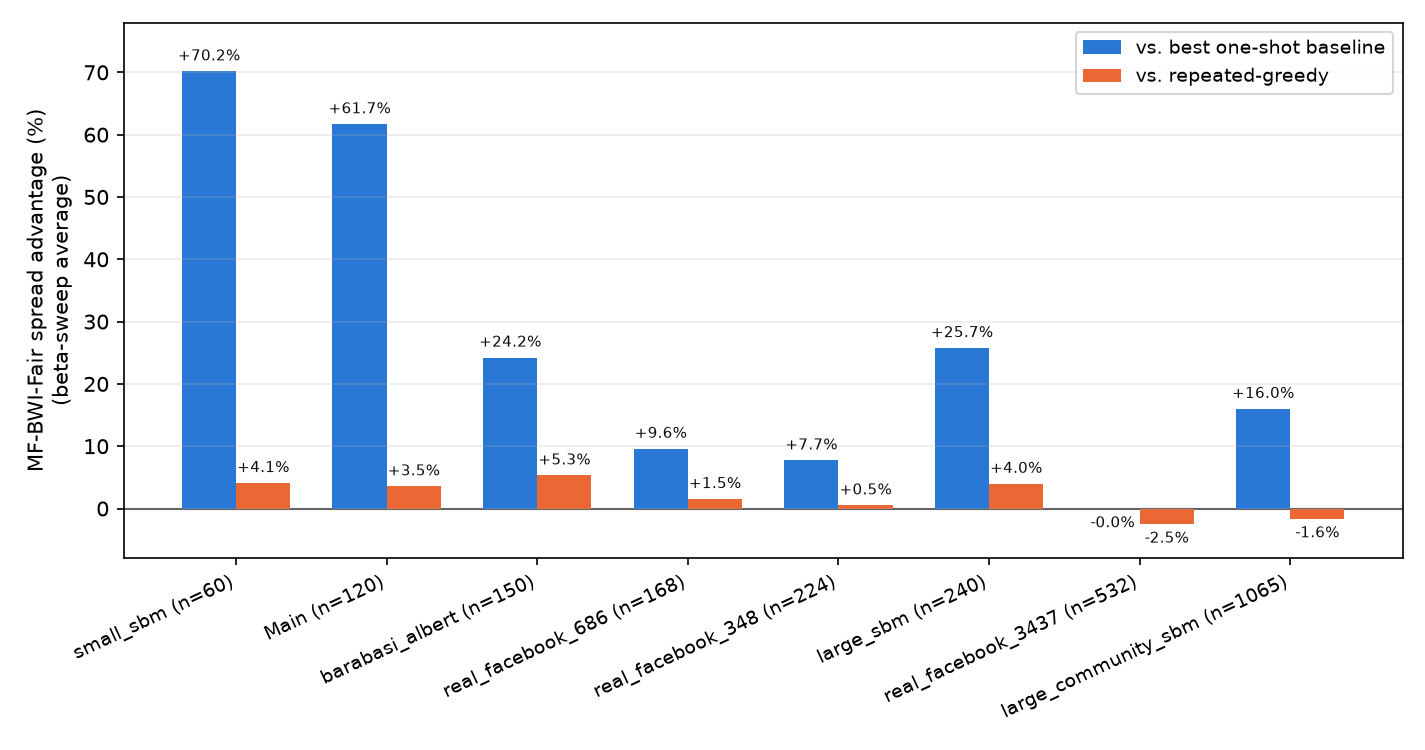
\includegraphics[width=\columnwidth]{figures/cross_graph_summary.png}
\caption{MF-BWI-Fair's mean spread advantage (\%) over the best one-shot
baseline and over repeated-greedy, averaged across each graph's own
$\beta$ sweep, for all eight graphs tested (synthetic and real, ordered
by node count).}
\label{fig:cross-graph}
\end{figure}

\begin{table}[t]
\centering
\caption{Real Facebook ego-network (\texttt{real\_facebook\_348}):
MF-BWI-Fair vs.\ repeated-greedy, reduced vs.\ full compute budget
(full-budget column post-harness-fix).}
\label{tab:realgraph}
\begin{tabular}{lcc}
\toprule
Checkpoint & Reduced budget & Full budget \\
\midrule
$\beta=0.0$, spread    & $-9.3\%$ & $-1.2\%$ (tied) \\
$\beta=0.5$, spread    & $-5.1\%$ & $\mathbf{+1.5\%}$ \\
$\beta=0.5$, min-reach & $-26\%$  & $\mathbf{+3.1\%}$ \\
$q=0.1$, spread        & $-4.2\%$ & $-0.2\%$ (tied) \\
$q=0.4$, spread        & $-2.3\%$ & $\mathbf{+2.7\%}$ \\
$q=0.4$, min-reach     & $+14\%$  & $\mathbf{+3.5\%}$ \\
\bottomrule
\end{tabular}
\end{table}

\subsection{Validation against the original authors' IMM implementation}
\label{sec:results-imm}

Every baseline reported above other than the classical objective forms
they target is this project's own reimplementation, not the original
authors' code (Section~\ref{sec:setup}). We benchmark our IMM
reimplementation~\cite{tang2015influence} directly against the original
authors' published C++ implementation on the main benchmark graph. The
two implementations select different-but-comparable seed sets (low
node-level overlap is expected on a small, community-structured graph
with substantial within-block redundancy), but land within 0.6\% of each
other's independently re-measured expected spread (32.08 vs.\ 32.27) and
within 2\% of CELF greedy's spread -- consistent with both legitimately
approximating the same submodular objective well, as IMM's
$(1-1/e-\varepsilon)$-approximation guarantee promises. No bug was found
in our IMM reimplementation during this exercise. As expected from IMM's
near-linear-time design, the original C++ binary is faster still than
our Python port at this graph's small scale (sub-millisecond vs.\ 0.019s),
both far faster than CELF's Monte Carlo greedy (1.8s); IMM's design
advantage is intended to show up at much larger scale than this
benchmark's 120 nodes.

\section{Discussion and Limitations}
\label{sec:limitations}

\textbf{Graph coverage remains limited, and the largest real network
tested shows a narrower, specifically-attributed exception.}
Section~\ref{sec:results-multigraph} shows that the main benchmark's
finding reproduces cleanly across two further synthetic scales and a
structurally different scale-free topology. It also reproduces against
every one-shot classical baseline on all three real social networks we
tested, in the same qualitative shape (tied at low backfire/recovery,
with a growing MF-BWI-Fair lead as either increases), but only once we
match compute budget to the main benchmark and fix a harness bug that
had given one-shot baselines an unearned propagation head start. Three
real networks is still a small sample, and all three are SNAP
ego-Facebook subgraphs. On the largest and sparsest of the three (532
nodes, 6 detected communities), MF-BWI-Fair trails one baseline,
repeated-greedy specifically, by a small, stable $\sim\!2.5$--$2.7\%$
mean spread margin. The harness fix does not change this margin, since
repeated-greedy receives the identical correction.

Two explanations for this residual gap compete. First, it could be a
genuine control-quality gap: repeated-greedy's expensive per-round
joint-rollout evaluation can capture community-bridging effects that
MF-BWI-Fair's cheaper, mean-field-decoupled Lagrangian index cannot.
Second, it could be a parameter-uncertainty cost: we deliberately hand
repeated-greedy the true diffusion parameters directly, as a
strong-baseline design choice (Section~\ref{sec:setup}), while
MF-BWI-Fair only ever sees its own Bayesian posterior estimates. We
distinguish the two with a direct ablation. We re-run MF-BWI-Fair on the
same graph with its Bayesian tracker bypassed and its own posterior
forced to the true parameters throughout, at 6 representative $\beta$/$q$
operating points and 5 trials each. This leaves the gap to
repeated-greedy statistically unchanged: the mean gap is $-2.60\%$ with
the Bayesian posterior (15 trials, same 6 points) and $-2.81\%$ with true
parameters (5 trials), a $-0.21$ percentage-point difference with an
approximate 95\% CI of $[-0.73,+0.31]$ -- crossing zero, and if anything
trending in the opposite direction from what the uncertainty-cost
explanation would predict. This ablation therefore finds no support for
the uncertainty-cost explanation and, by elimination, favors the first:
the residual gap looks like a genuine control-quality effect of the
mean-field-decoupled index rather than a cost of not knowing the true
parameters. It is not, on its own, a controlled test of density or
degree as confounds -- the smaller, denser 348-node and 686-node graphs
simply show no such gap against any baseline, including repeated-greedy,
which argues against density/degree alone as a simple, monotonic driver
across the three real graphs tested, though (as the next paragraph
finds) it does not yet isolate density's possible interaction with
\texttt{real\_facebook\_3437}'s specific community structure.

What structural property of \texttt{real\_facebook\_3437} drives it is
less clear than a first look suggests. The natural candidate --
that six disparately-sized communities are simply harder for mean-field
decoupling as a network grows -- is directly testable by scaling that
same structure up on a synthetic graph, so we built one:
\texttt{large\_community\_sbm}, a stochastic block model with
\texttt{real\_facebook\_3437}'s own six community-size ratios
(165:137:79:42:39:70) scaled to twice its node count ($n=1{,}065$), at a
modest average degree ($\approx\!9.7$) comparable to the other synthetic
checks above rather than to \texttt{real\_facebook\_3437}'s own denser
topology ($\approx\!36$). MF-BWI-Fair beats every one-shot baseline by a
wide margin at every point of both sweeps on this graph, exactly as
everywhere else, but the gap to repeated-greedy neither reproduces nor
grows: pooled across all 8 sweep points (6 trials each), the mean gap is
$-1.05\%$ (95\% CI $[-1.74\%,-0.36\%]$), smaller than
\texttt{real\_facebook\_3437}'s $-2.5$--$2.7\%$, individually
indistinguishable from zero at 5 of 8 points, and it even flips sign at
the highest recovery rate tested ($q=0.4$: $+1.81\%$, CI crossing zero)
(Figure~\ref{fig:large-community-sweeps}). Scaling the same
community-size ratio up, at a typical synthetic density, is therefore
not on its own sufficient to reproduce \texttt{real\_facebook\_3437}'s
gap. Graph density, or some other property specific to that one real
network, remains a live alternative we have not yet isolated. Broader
real-network coverage beyond the ego-Facebook family, and a
density-matched (rather than community-ratio-matched) synthetic test,
remain future work.

\begin{figure}[t]
\centering
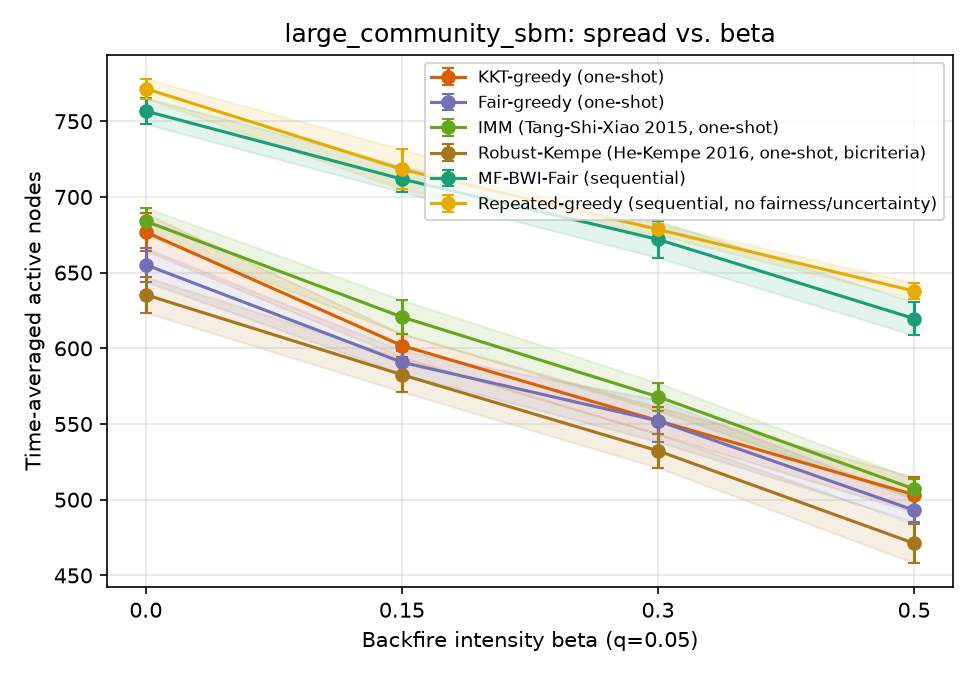
\includegraphics[width=\columnwidth]{figures/large_community_sbm_beta.png}
\\[4pt]
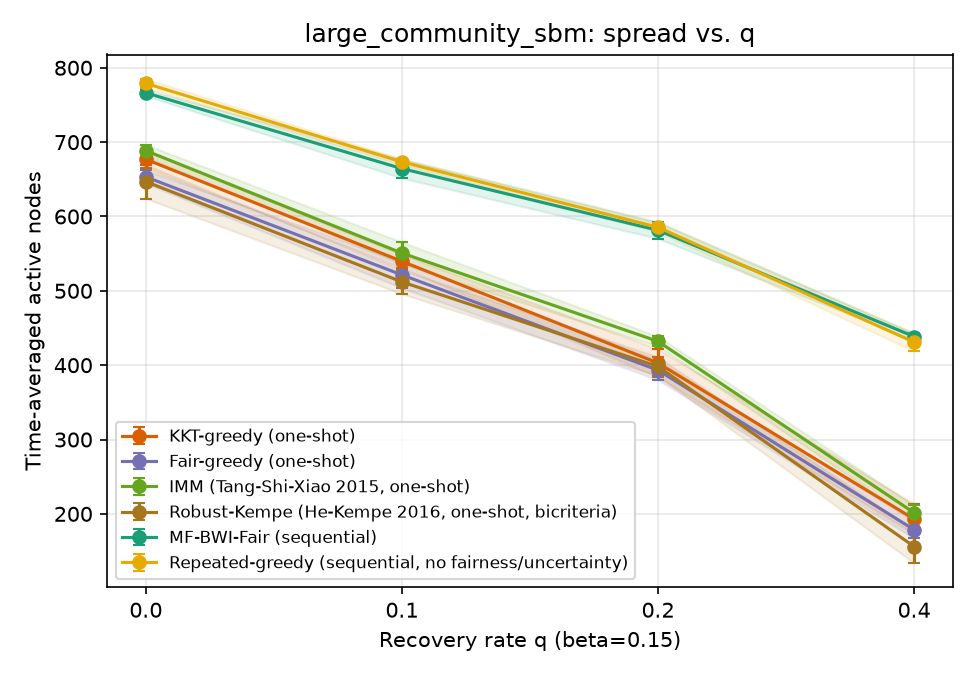
\includegraphics[width=\columnwidth]{figures/large_community_sbm_q.png}
\caption{\texttt{large\_community\_sbm} (1,065 nodes, six community
sizes scaled from \texttt{real\_facebook\_3437}): time-averaged spread
vs.\ backfire intensity $\beta$ at $q=0.05$ (top) and vs.\ recovery rate
$q$ at $\beta=0.15$ (bottom), mean $\pm$ 95\% CI shading, 6 trials per
point. MF-BWI-Fair (teal) leads every one-shot baseline throughout and
tracks repeated-greedy (yellow) closely, unlike the stable, one-sided
gap seen on \texttt{real\_facebook\_3437} itself.}
\label{fig:large-community-sweeps}
\end{figure}

\textbf{A further backfire-dependent hardness worsening remains an open
conjecture, deliberately not claimed as a result.} A candidate constant
$c(\beta)\ge0.94$ (Section~\ref{sec:hardness}) would
follow from one extra property of Feige's hard instances -- that the
fraction of elements covered exactly once by any candidate solution is
bounded by roughly $1/e$ -- which is plausible (a concentration argument
over Feige's random-partition construction) but requires two technical
steps we have not both closed: (i) a concavity property of
$d\mapsto\mathbb{E}\,\varphi_\beta(\mathrm{Bin}(d,1/k))$, where
$\varphi_\beta(c)=1/(2-(1-\beta)^c)$ is the exact per-element value
function from Theorem~\ref{thm:hardness}'s proof; (ii) a cross-term
pairwise-soundness property of the same reduction, re-verified for this
statistic rather than for plain coverage. We checked (i) numerically --
exhaustively across $\beta\in[0.01,0.99]$ and $k\in\{2,\dots,200\}$, it
holds for every degree $d\le k$ (the regime Feige's construction uses) and
only fails for $d\gtrsim4k$, well outside that regime -- which is genuine
evidence, not a proof, since it does not establish the claim analytically
and (ii) is a separate, deeper re-derivation of part of Feige's reduction
that we have not attempted to a publishable standard. We therefore report
this only as a conjecture with supporting structural evidence (the
per-edge revive-at-least-as-fast-as-kill asymmetry noted in
Section~\ref{sec:hardness}, and several natural gadget constructions all
failing to encode a hard-to-decide dependence on the seed set) and the
numerical check above, not as a theorem or a proposition of this paper.

\textbf{No comparison against the original authors' code for He--Kempe or
Rahmattalabi et al.} Neither paper has published code corresponding to the
specific algorithm reimplemented here (a superficially related repository
for Rahmattalabi et al.\ in fact implements a different paper,
Tsang et al.~\cite{tsang2019group}, and must not be conflated with it).
Only IMM has verifiable original code; Section~\ref{sec:results-imm}
reports a direct benchmark against it and finds our reimplementation
trustworthy, but this does not extend to He--Kempe or Rahmattalabi et
al., whose reported numbers here remain characterizations of independent
reimplementations only.

\textbf{The mean-field approximation's own error is not separately
quantified.} The belief fixed point of Section~\ref{sec:algorithm} is an
approximation whose deviation from the true (intractable) joint
activation distribution has not been bounded or measured in isolation from
the end-to-end policy's performance; this is a natural target for future
analysis.

\textbf{The sandwich bound is demonstrably loose, and this is a direction,
not a hidden flaw.} Exact computation on small instances (2--8 nodes,
$T\sim300$) shows the sandwich ratio $\rho$ loose by up to an order of
magnitude where it applies at all (e.g., roughly $13\times$ on a directed
star instance, because the lower surrogate inflates every node's recovery
uniformly by $\delta_v$ even where a node has no active in-neighbor left),
and vacuous whenever $q=0$ or $q+\beta\Delta_{\mathrm{in}}\ge1$. Separately,
$f_\beta/f_0$ is not bounded below by any instance-independent constant (a
bidirected $K_6$ instance at $\beta=0.5,q=0.05$ collapses by a factor of
roughly $300\times$ relative to $f_0$), so no purely multiplicative
comparison against $f_0$ can be the source of a strong general guarantee.
Yet greedy run on the plain $\beta=0$ surrogate landed within 1\% of
$\mathrm{OPT}_\beta$ on every one of the six small instances tested --
suggestive, not proof, that the practical quality of surrogate-greedy
substantially exceeds what $\rho(1-1/e)$ certifies. We read this as the
concrete next step for this line of work: a sharper \emph{upper}-bound
analysis (a per-instance or instance-class argument in the spirit of the
exact layered value formula behind Theorem~\ref{thm:hardness}), rather
than a search for a matching lower bound on $\rho$ itself, which the
evidence here suggests is not the right quantity to target.

\textbf{Indexability is checked, not proven.} As stated in
Proposition~\ref{prop:indexability}, the down-set property underlying the
closed-form index's exactness is verified numerically on random instances
over a fine $\lambda$ grid, not established as a general theorem for this
2-state/3-action case.

\textbf{An open, unconditional route to a matching lower bound.} We
identify, but do not pursue to completion, a possible unconditional
alternative to the conjectured constant above: the class of functions
$S\mapsto\sum_v\varphi(c_v(S))$ is closed under the same symmetrization
used in Vondr{\'a}k's symmetry-gap framework~\cite{vondrak2013symmetry},
and the symmetric-instance gap for $\varphi_\beta$
(Theorem~\ref{thm:hardness}'s proof) works out numerically close to, and
slightly below, our conjectured $c(\beta)$. Whether Vondr{\'a}k's
smoothing-step argument -- which uses submodularity directly -- extends to
this non-submodular but structured class is open and was not checked; if
it does, it would give an unconditional oracle-model lower bound without
needing the unverified property the conjecture above depends on. We flag
this as the single most promising next step toward a proof, should this
line of work be pursued further.

\section{Conclusion}

This paper formalized a combined relaxation of the four assumptions
behind the classical influence-maximization guarantee: progressive
dynamics, monotone submodularity, known parameters, and fairness-free
objectives. We proved that a sandwich approximation recovers a
$\rho(1-1/e)$ guarantee for every backfire intensity, and we gave a
closed-form index that makes the resulting control problem tractable at
near-linear per-round cost. We proved that $(1-1/e)$-hardness survives
backfire exactly, and we explicitly declined to upgrade a plausible but
unproven constant-factor worsening result to theorem status. We also
corrected a measured fairness pathology in an existing welfare objective
and implemented the result in MF-BWI-Fair.

On the main benchmark, MF-BWI-Fair matches or exceeds every tested
baseline, including independently-verified published algorithms, in both
spread and fairness, and this finding reproduces across three further
synthetic graphs spanning two scales and a structurally different
topology. On three real social networks tested at increasing scale, the
finding initially did not hold. We traced this to two distinct causes: a
necessarily reduced compute budget, and a harness bug that gave one-shot
baselines an unearned one-round propagation head start over the two
sequential methods. Fixing both restores MF-BWI-Fair's lead over every
one-shot classical baseline at all three real-graph scales, with one
exception discussed in Section~\ref{sec:limitations}. Testing on real
networks beyond the ego-Facebook family used here remains open for
future work. We also directly validated our IMM reimplementation
against the original authors' C++ code and found it trustworthy.

\bibliographystyle{IEEEtran}
\bibliography{references}

\end{document}
